\documentclass[a4paper]{article}
\usepackage[english]{babel}
\usepackage[utf8x]{inputenc}
\usepackage{amsmath}
\usepackage{graphicx}
\usepackage[colorinlistoftodos]{todonotes}
\usepackage{listings}
\usepackage{cite}
\usepackage{glossaries}
\usepackage[
top    = 2.75cm,
bottom = 2.00cm,
left   = 2.50cm,
right  = 2.00cm]{geometry}

\title{Remoting Patterns}

\author{Martin Haidn \& Hannah Siegel}

\date{\today}

\begin{document}
\maketitle
\newpage

\tableofcontents
\newpage

\section{Aufgabenstellung}
Gruppenarbeit: 2 Mitglieder (Server/Client)\\
\\
Analysieren Sie in einer Gruppe von 2 Leuten die mitgelieferte Implementation der verteilten LeelaApplikation. Identifizieren Sie dabei alle verwendeten Elemente der "Basic Remoting Patterns" und erstellen Sie UML-Klassendiagramme für die Pakete comm, comm.socket, comm.soap, evs2009 und evs2009.mapping.\\
Schließen Sie die unfertigen Tests ab, und dokumentieren Sie etwaige Schwierigkeiten.\\
\\
\textbf{Was ist zu tun?}
\begin{itemize}
	\item UML Klassendiagramm
	\item Erweitern der Testfälle (mind. einen Testfall erweitern)
	\item Kritik und Verbesserungsvorschläge
\end{itemize}
\mbox{} \\
\textbf{Punkte (16):}\\
Identifikation von Basic Remoting Patterns ... 1Pkt\\
Beschreibung der Applikation ... 4Pkt\\
UML-Diagramme ... 3Pkt\\
Schreiben von einem neuen Testfall ... 2Pkt\\
konstruktive Verbesserungsvorschläge / Kritikpunkte ... 6Pkt\\
\\
\textbf{Main-Method-Classes}\\
\begin{center}
	\begin{tabular}{ | r | r |}
		\hline
		SOAPPluginServer & src/main/java/comm/soap/SOAPPluginServer.java \\
		\hline
		Application & src/main/java/evs2009/Application.java \\
		\hline
	\end{tabular}
\end{center}
\section{Arbeitszeit}
Die Arbeitszeit ist in diesem Falle nicht auf die Personen aufgeteilt, weil immer gleich lange gearbeitet wurde.
\subsection{Abschaetzung}
\begin{center}
  \begin{tabular}{ | p{0.4\textwidth} |  p{0.4\textwidth}|}
    \hline
    \textbf{Aufgabe} & \textbf{Zeit} (in minuten) \\ 
    \hline 
    \hline
    Applikation zum Laufen bringen & 60 \\ 
    \hline
    Identifikation von Basic Remoting Patterns & 30 \\ 
    \hline
  	Beschreibung der Applikation & 60 \\ 
    \hline
  	UML-Diagramme & 60 \\ 
    \hline
    Schreiben von einem neuen Testfall & 30 \\ 
    \hline
    konstruktive Verbesserungsvorschläge / Kritikpunkte & 60 \\ 
    \hline
   Dokumentation & 60 \\ 
    \hline
    \hline
    Total & 6 Stunden \\

    \hline
  \end{tabular}
\end{center}
\begin{center}
  \begin{tabular}{ | p{0.4\textwidth} |  p{0.4\textwidth}|}
    \hline
    \textbf{Aufgabe} & \textbf{Zeit} (in minuten) \\ 
    \hline 
    \hline
    Applikation zum Laufen bringen & 180 \\ 
    \hline
    Identifikation von Basic Remoting Patterns & 60 \\ 
    \hline
  	Beschreibung der Applikation & 60 \\ 
    \hline
  	UML-Diagramme & 30 \\ 
    \hline
    Schreiben von einem neuen Testfall & 90 \\ 
    \hline
    konstruktive Verbesserungsvorschläge / Kritikpunkte & 60 \\ 
    \hline
   Dokumentation & 60 \\ 
    \hline
    \hline
    Total & 9 Stunden \\
    \hline
  \end{tabular}
\end{center}
\newpage
\section{Einleitung}
\subsection{Allgemein}
Design Patterns haben in den letzten Jahren eine bedeutende Rolle in der objektorientierten\\
Softwareentwicklung bekommen.\\
Ein Pattern ist mit einer Drei-Punkte-Regel zu vergleichen und setzt sich aus den folgenden Komponenten zusammen:
\begin{itemize}
	\item Kontext
	\item Problem
	\item Lösung
\end{itemize}
Ziel und Nutzen eines Patterns soll es sein Software zu entwickeln, der es möglich ist sich soweit selbst zu konfigurieren,
dass interne Prozesse auf ein sich änderndes Umfeld angepasst und optimiert werden können.\\
\subsection{Verteilte Systeme}
Im gebiet der verteilten Systeme kommen allerdings ein paar weiterte Herausforderungen auf uns zu.\\
Folgenden Herausforderungen schenken wir hierbei unser Augenmerk:
\begin{itemize}
	\item Network Latency
	\item Predictability
	\item Concurrency
	\item Scalability
	\item Partial Failure
\end{itemize}
\begin{figure}[here!]
	\centering	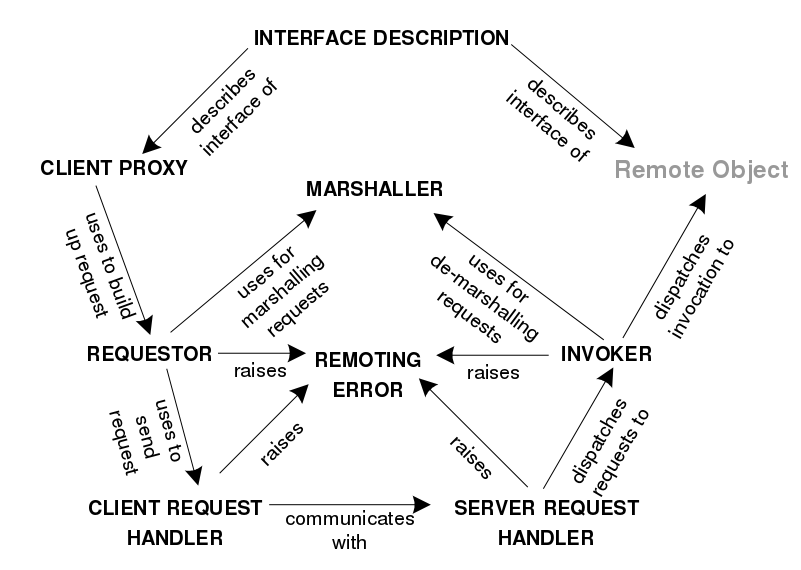
\includegraphics[scale=0.4]{remoting_patterns.png}
\caption{Remoting Patterns}
	\end{figure}
    Die dick gedruckten Knotenpunkte in der obigen Grafik, beschreiben bereits unsere Remoting Patterns.\\
Im Zuge dieser Übung haben wir uns mit dem LeelaApplikation-Framework auseinandergesetzt und den Code auf Basic Remoting Patterns untersucht.\\
Eine detailierte Übersicht folgt im nächsten Punkt.
\cite{martin}
\subsection{Identifikation Basic Remoting Patterns}
\begin{center}
	\begin{tabular}{ | p{0.4\textwidth} | p{0.4\textwidth} |}
		\hline
		Pattern & Klasse(n) welche dieses implementieren \\
		\hline \hline
		Interface Description &  z.B. Peer  \\
		\hline
        Marshaller &  zwar heisst eine Klasse XMLMarshaller, diese ist allerdings leer. \\
		\hline
        Remoting Error & EppErrorCode und EppErrorException \\
		\hline
        Remote Object &  z.B. Client Peer\\
		\hline
        Server Request Handler & Request Handler \\
		\hline
          Client Request Handler &  Request Handler\\
		\hline
          Requestor & Requestor \\
		\hline
          Client Proxy &  \\
		\hline
         Invoker & Interface: Invoker - SocketPluginServer \& SOAPPluginServer haben zwar ein Invoker object. Wir konnten leider keine Klasse finden, welche das Invoker Interface konkret implementiert. \\
		\hline
	\end{tabular}
\end{center}
\section{Beschreibung der Applikation}
Die Hauptklasse des Programmes stellt \textbf{Application.java} dar, in der über den PeerReader alle Peer-ID's und die dazugehörigen Adressen eingelesen werden
Für den lokalen Test der Applikation wurden diese Adressen auf "localhost" gesetzt. Es werde n entweder Sockets oder SOAP verwendet, je nach dem, welches Protokoll der Endpoint des beim starten angegebenen Peers verwendet.  Danach wird das Programm so richtig gestartet, indem vom RequestHandler der Invoker und der Requestor gestartet werden. Ueber die Plugins, welche ja bestimmen welche Protokolle verwendet werden wird anscheinend ueber die methoden getServer() und getClient() alles gestartet. Die methoden getServer() und getClient() werden vom Interface ProtocolPlugin vorgezeichnet und dann von den konkreten Implementationen, beispielsweise SOAPPluginServer, implementiert.
Der peer wird beim RequestHandler registriert.
Weiters wird die ServerPeerImplementaion verwendet, um anschliessend das Verschicken von byte streams zu simulieren. \\
Auch wenn dieses Beispiel nicht ganz klar zu verfolgen ist, und uns nicht immer zu hundert Prozent klar ist, wo und vorallem warum alles so funktioniert, konnten wir sehr deutlich Remoting Patterns erkennen.
\newpage
\section{UML}
Eine Bessere Qualitaet der Diagramme finden sich in der Abgabe. \\ Sie wurden mittels Astah generiert. 
	\subsection{comm}
	\begin{figure}[here!]
	\centering
	\includegraphics[width=1.0\textwidth]{comm.png}
	\caption{UML of the comm package}
	\end{figure}
    \newpage
	\subsection{comm.socket}
	\begin{figure}[here!]
	\centering
	\includegraphics[width=1.0\textwidth]{client.png}
	\caption{UML of the soap package}
	\end{figure}
	\subsection{comm.soap}
	\begin{figure}[here!]
	\centering
	\includegraphics[width=1.0\textwidth]{socket.png}
	\caption{UML of the socket package}
	\end{figure}

\newpage
\subsection{evs und evs.mapping}
Die Autogenerierten UMLs sind hierbei leider absolut nicht brauchbar. Die generierten UMLs sind in der Abgabe zu finden. Die autogenerierten UMLs spiegeln nicht den Soll-Zustand wieder. Wir haben die git history reverted und daher ein Protokoll bekommen. Dort sind sehr gute UMLs zu finden anhand denen man sehr viel erfahren kann.  
\section{Testfälle}
\subsection{Vorhandene Testfaelle}
Ganz am Anfang wollten wir alle Tests laufen lassen, um auf einen Blick sehen zu koennen, an welchen Stellen noch keine gute Abdeckung erzielt wurde. Daher haben wir eine Klasse AllTests erstellt mit welcher wir alle Tests auf einmal laufen lassen wollten.\\
Es gibt insgesammt 25 Tests, wobei die wenigsten von ihnen funktioniert haben - es wurden unter anderem laufend exceptions geworfen. Die Tests haben allerdings einzeln besser funktioniert. Ohne etwas am code zu veraendern, hatten wir unterschiedliche Ergebniss je nach dem in welcher Reihenfolge und in welchem Kontext die Tests aufgerufen wurden. Das zeugt nicht gerade von guten Tests, allerdings waren wenigstens welche vorhanden.
\begin{figure}[here!]
	\centering
	\includegraphics[width=0.6\textwidth]{screenshot1.png}
	\caption{Funktionierender ApplicationTest wenn einzeln aufgerufen}
	\end{figure}
    
    \begin{figure}[here!]
	\centering
	\includegraphics[width=0.6\textwidth]{generasltestsfails1.png}
	\caption{Nicht funktionierender ApplicationTest wenn gesammt aufgerufen}
	\end{figure}
     
\subsection{Hinzufuegen eines Testfalles}
Das Hinzufuegen eines Tesfalles ging sich leider nicht mehr aus. 
\newpage
\section{Kritik und Verbesserungsvorschläge}
\begin{itemize}
\item \textbf{Keinerlei Dokumentation} \\ 
Es sind keinerlei Kommentare (von Inlinekommentaren mal ganz abgesehen, nichtmal methoden oder Klassenkommentare!). Wir verwenden schon ungerne APIs, welche nicht ausreichend kommentiert sind - geschweige denn gar nicht. Eine nicht dokumentierte Software ist daher einfach nicht brauchbar. 
\item \textbf{Testcases} \\
Die Testcases failen teilweise, aber wenigstens sind welche vorhanden.
\item \textbf{Exceptionhandling} \\
Das Exceptionhandling ist allgemein eher sehr spaerlich. Man kann zum Beispiel eine ArrayIndexOutOfBounds Exception schmeissen lassen, wenn man das Programm ohne Programmparametern startet. \\ 
Allerdings moechten wir auch darauf Hinweisen, dass eine try-catch statement welche einfach nur eine 'Exception e' auffaengt in dem Konstruktor der Startklasse zu finden ist.  
\item \textbf{Start} \\
Usage Application <namelist> <peerId> ist ja wohl foellig falsch.
\item \textbf{Komplexer Code}\\
Der Code ist etwas komplex, und jedoch unterstuetzt er trotzdem nur SOAP und Sockets. 
\item \textbf{Nicht implementierter Code}\\
Interfaces werden nicht alle verwendet, login und logout funktion nicht verwendet und der gesammte Code scheint keinen augenscheinlichen Nutzen zu haben ...
\item \textbf{Programmaufruf funktioniert nicht}\\
Der Programmaufruf mit einem Argument, naemlich einer ID eines Peers funktioniert trotzdem nicht
\item \textbf{Benuertzung eines Patterns - bennenung wie pattern}\\
Der Sinn hinter der Benuetzung eines Pattern, ist unter anderem auch, dass andere Programmierer sich schneller zurechtfinden. Dies waere hier in diesem Falle vielleicht ganz angebracht gewesen. Dh die Klassen nach ihren Funktionen laut dem Basic Remoting Pattern benennen.
\item \textbf{Organisation der Klassen}\\
Die Packages machen eher wenig sinn (evs2009?). Eine bessere Verwaltung der packages kann durchaus sinnvoll sein.
\item \textbf{Verwendung eines funktionierendes(!) Buildtools}\\
Builden mittels ant funktioniert leider nicht. Das File ist auch irgendwie zu leer.

\end{itemize}

\newpage
\listoffigures

\begin{thebibliography}{56}

\bibitem{martin}
	\textbf{Remoting Patterns} \\
   Uwe Zdun, Markus Völter, Michael Kircher\\
  \emph{Online: 	http://nm.wu-wien.ac.at/research/publications/b375.pdf}\\
  called up: 02.10.2014 22:53

\bibitem{borkoprotokoll}
	\textbf{Lightweight Leela1 SOA Middleware
Communication Framework} \\
  Borko Michael,Greifeneder Michael,Motlik Florian \\
  \emph{Online: 	http://stackoverflow.com/questions/822323/how-to-generate-a-random-number-in-c}\\
  called up: 28.09.2014 12:00
  
  \bibitem{junit}
	\textbf{Stack Overflow} \\
   ashu, answered Sep 12 '11 at 12:46\\
  \emph{Online: 	http://stackoverflow.com/questions/1070202/junit-suiteclasses-with-a-static-list-of-classes}\\
  called up: 02.10.2014 21:023

\end{thebibliography}             

\end{document}
